\documentclass[aspectratio=169]{beamer}
\mode<presentation>
\usetheme{Hannover}
\useoutertheme{sidebar}
\usecolortheme{dolphin}

\usepackage{amsmath}
\usepackage{amssymb}
\usepackage{enumerate}


% some bold math symbosl
\newcommand{\Cov}{\mathrm{Cov}}
\newcommand{\Cor}{\mathrm{Cor}}
\newcommand{\Var}{\mathrm{Var}}
\newcommand{\brho}{\boldsymbol{\rho}}
\newcommand{\bSigma}{\boldsymbol{\Sigma}}
\newcommand{\btheta}{\boldsymbol{\theta}}
\newcommand{\bbeta}{\boldsymbol{\beta}}
\newcommand{\bmu}{\boldsymbol{\mu}}
\newcommand{\bW}{\mathbf{W}}
\newcommand{\one}{\mathbf{1}}
\newcommand{\bH}{\mathbf{H}}
\newcommand{\by}{\mathbf{y}}
\newcommand{\bolde}{\mathbf{e}}
\newcommand{\bx}{\mathbf{x}}

\newcommand{\cpp}[1]{\texttt{#1}}

\title{Mathematical Biostatistics Boot Camp: Lecture 12, Bootstrapping}
\author{Brian Caffo}
\date{\today}
\institute[Department of Biostatistics]{
  Department of Biostatistics \\
  Johns Hopkins Bloomberg School of Public Health\\
  Johns Hopkins University
}


\begin{document}

\frame{\titlepage}


\section{Table of contents}
\frame{
  \frametitle{Table of contents}
  \tableofcontents
}

\section{The jackknife}
\begin{frame}\frametitle{The jackknife}
\begin{itemize}
\item The jackknife is a tool for estimating standard errors 
  and the bias of estimators 
\item As its name suggests, the jackknife is a small, handy tool; in contrast to
  the bootstrap, which is then the moral equivalent of a
  giant workshop full of tools
\item Both the jackknife and the bootstrap involve {\em resampling}
  data; that is, repeatedly creating new data sets from the original
  data
\end{itemize}
\end{frame}

\begin{frame}\frametitle{The jackknife}
  \begin{itemize}
\item The jackknife deletes each observation and calculates an estimate
  based on the remaining $n-1$ of them
\item It uses this collection of estimates to do things like estimate
  the bias and the standard error
\item Note that estimating the bias and having a standard error are
  not needed for things like sample means, which we know are unbiased
  estimates of population means and what their standard errors are
  \end{itemize}
\end{frame}

\begin{frame}\frametitle{The jackknife}
  \begin{itemize}
  \item We'll consider the jackknife for univariate data
  \item Let $X_1,\ldots,X_n$ be a collection of data used to estimate
    a parameter $\theta$
  \item Let $\hat \theta$ be the estimate based on the full data set
  \item Let $\hat \theta_{i}$ be the estimate of $\theta$ obtained by
    {\em deleting observation $i$}
  \item Let $\bar \theta = \frac{1}{n}\sum_{i=1}^n \hat \theta_{i}$
  \end{itemize}  
\end{frame}

\begin{frame}\frametitle{Continued}
  \begin{itemize}
 \item Then, the jackknife estimate of the bias is
   $$
   (n - 1) \left(\bar \theta - \hat \theta\right)
   $$
   (how far the average delete-one estimate is from the actual estimate)
 \item The jackknife estimate of the standard error is
   $$
   \left[\frac{n-1}{n}\sum_{i=1}^n (\hat \theta_i - \bar\theta )^2\right]^{1/2}
   $$
   (the deviance of the delete-one estimates from the average delete-one estimate)
  \end{itemize}
\end{frame}

\begin{frame}\frametitle{Example}
\begin{itemize}
\item Consider the data set of $630$ measurements of gray matter volume
  for workers from a lead manufacturing plant
\item The median gray matter volume is around 589 cubic centimeters
\item We want to estimate the bias and standard error of the median
\end{itemize}
\end{frame}

\begin{frame}[fragile]\frametitle{Example}
The gist of the code
\begin{verbatim}
n <- length(gmVol)
theta <- median(gmVol)
jk <- sapply(1 : n,
             function(i) median(gmVol[-i])
             )
thetaBar <- mean(jk)
biasEst <- (n - 1) * (thetaBar - theta) 
seEst <- sqrt((n - 1) * mean((jk - thetaBar)^2))
\end{verbatim}
\end{frame}

\begin{frame}[fragile]\frametitle{Example}
Or, using the \texttt{bootstrap} package
\begin{verbatim}
library(bootstrap)
out <- jackknife(gmVol, median)
out$jack.se
out$jack.bias
\end{verbatim}
\end{frame}

\begin{frame}\frametitle{Example}
  \begin{itemize}
  \item Both methods (of course) yield an estimated bias of $0$ and a
    se of $9.94$
  \item Odd little fact: the jackknife estimate of the bias for the
    median is always $0$ when the number of observations is even
  \item It has been shown that the jackknife is a linear approximation to
    the bootstrap
  \item Generally do not use the jackknife for sample quantiles like the median;
    as it has been shown to have some poor properties
  \end{itemize}
\end{frame}

\begin{frame}\frametitle{Pseudo observations}
  \begin{itemize}
    \item Another interesting way to think about the jackknife uses pseudo observations
    \item Let
      $$
      \mbox{Pseudo Obs} = n \hat \theta - (n - 1) \hat \theta_{i}
      $$
    \item Think of these as ``whatever observation $i$ contributes to the estimate of $\theta$''
    \item Note when $\hat \theta$ is the sample mean, the pseudo observations are the data themselves
    \item Then the sample standard error of these observations is the previous jackknife estimated standard error.
    \item The mean of these observations is a bias-corrected estimate of $\theta$
  \end{itemize}
\end{frame}

\section{The bootstrap principle}
\begin{frame}\frametitle{The bootstrap}
\begin{itemize}
\item The bootstrap is a tremendously useful tool for constructing
  confidence intervals and calculating standard errors for difficult
  statistics
\item For example, how would one derive a confidence interval for
  the median?
\item The bootstrap procedure follows from the so called bootstrap
  principle
\end{itemize}
\end{frame}

\begin{frame}\frametitle{The bootstrap principle}
\begin{itemize}
\item Suppose that I have a statistic that estimates some population
  parameter, but I don't know its sampling distribution
\item The bootstrap principle suggests using the distribution defined
  by the data to approximate its sampling distribution
\end{itemize}
\end{frame}

\section{The bootstrap}
\begin{frame}\frametitle{The bootstrap in practice}
\begin{itemize}
\item In practice, the bootstrap principle is always carried out
  using simulation
\item We will cover only a few aspects of bootstrap resampling
\item The general procedure follows by first simulating complete data sets
  from the observed data with replacement
  \begin{itemize}
  \item This is approximately drawing from the sampling distribution
    of that statistic, at least as far as the data is able to
    approximate the true population distribution
  \end{itemize}
\item Calculate the statistic for each simulated data set
\item Use the simulated statistics to either define a confidence interval
  or take the standard deviation to calculate a standard error
\end{itemize}
\end{frame}

\begin{frame}\frametitle{Example}
\begin{itemize}
\item Consider again, the data set of $630$ measurements of gray matter volume
  for workers from a lead manufacturing plant
\item The median gray matter volume is around 589 cubic centimeters
\item We want a confidence interval for the median of these
  measurements
\end{itemize}
\end{frame}

\begin{frame}
\begin{itemize}
\item Bootstrap procedure for calculating confidence interval for the median from a data
  set of $n$ observations
  \begin{enumerate}[$i.$]
  \item Sample $n$ observations {\bf with replacement} from the observed
    data resulting in one simulated complete data set
  \item Take the median of the simulated data set
  \item Repeat these two steps $B$ times, resulting in $B$ simulated
    medians
  \item These medians are approximately drawn from the sampling distribution
    of the median of $n$ observations; therefore we can
    \begin{itemize}
    \item Draw a histogram of them
    \item Calculate their standard deviation to estimate the standard error
      of the median
    \item Take the $2.5^{th}$ and $97.5^{th}$ percentiles as a confidence interval
      for the median
    \end{itemize}
  \end{enumerate}
\end{itemize}
\end{frame}

\begin{frame}[fragile]\frametitle{Example code}
\begin{verbatim}
B <- 1000
n <- length(gmVol)
resamples <- matrix(sample(gmVol,
                           n * B,
                           replace = TRUE),
                    B, n)
medians <- apply(resamples, 1, median)
sd(medians)
[1] 3.148706
quantile(medians, c(.025, .975))
    2.5%    97.5% 
582.6384 595.3553 
\end{verbatim}
\end{frame}

\begin{frame}
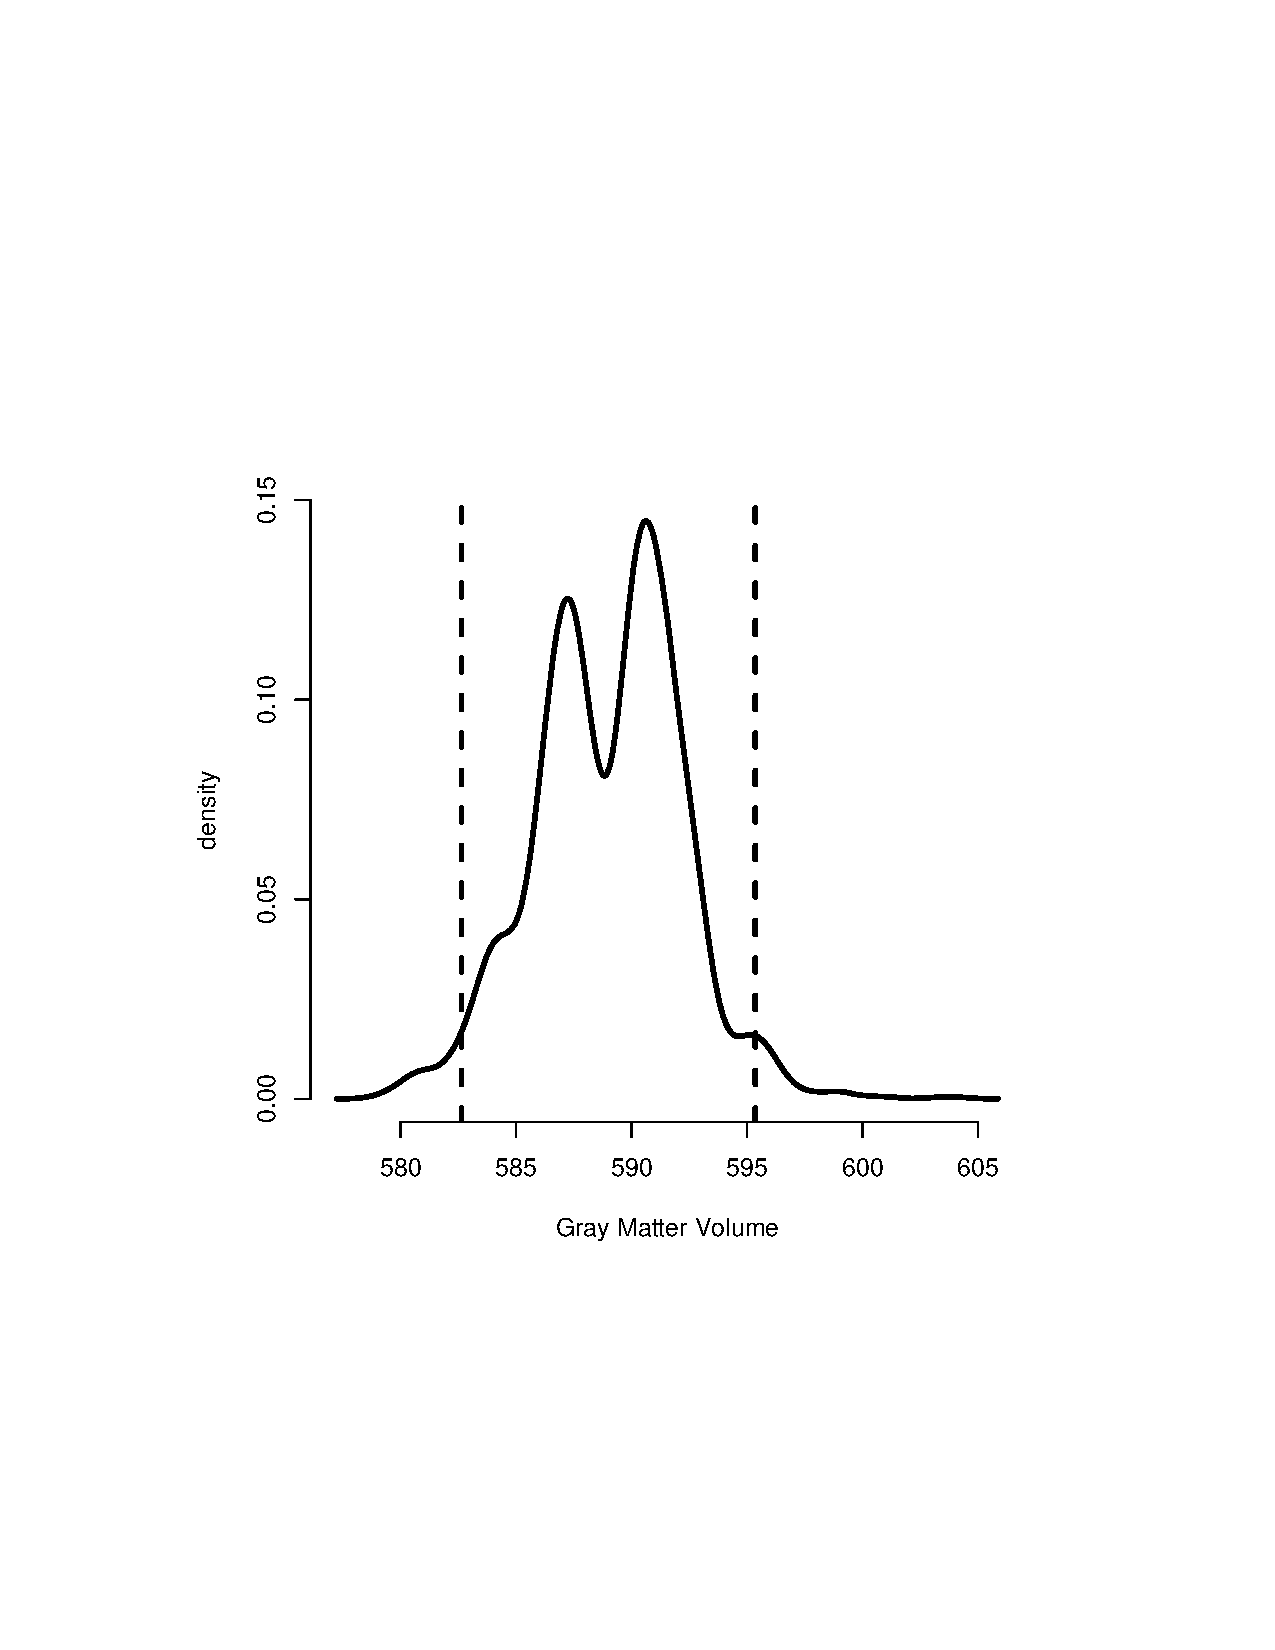
\includegraphics[width=3.5in]{bootstrap.pdf}
\end{frame}

\begin{frame}\frametitle{Notes on the bootstrap}
\begin{itemize}
\item The bootstrap is non-parametric
\item However, the theoretical arguments proving the validity of the
  bootstrap rely on large samples
\item Better percentile bootstrap confidence intervals correct for bias
\item There are lots of variations on bootstrap procedures; the book
  ``An Introduction to the Bootstrap'' by Efron and Tibshirani is a
  great place to start for both bootstrap and jackknife information
\end{itemize}
\end{frame}

\begin{frame}[fragile]
\begin{verbatim}
library(boot)
stat <- function(x, i) {median(x[i])}  
boot.out <- boot(data = gmVol,
                 statistic = stat,
                 R = 1000)
boot.ci(boot.out)
Level     Percentile            BCa          
95%   (583.1, 595.2 )   (583.2, 595.3 )  
\end{verbatim}
\end{frame}
\end{document}

